\chapter{PROPOSTA EXPERIMENTAL}
\label{chp:experiments}

Para o estudo em questão, propõe-se três experimentos que avaliarão tanto a capacidade de generalização do modelo de comparação de \textit{embeddings} quanto sua eficácia no problema de busca de código-fonte a partir de linguagem natural. As descrições e objetivos de cada experimento estão nas seções seguintes deste capítulo.

\section{Experimento 1}
\label{sec:experiments:experiment-1}
O objetivo desse experimento é determinar a capacidade de generalização do modelo de comparação.

Para tanto, foram utilizados os 100 primeiros pares código-fonte/comentário da base de treinamento. Para cada par p, removeu-se uma palavra aleatória do comentário, gerando uma \textit{query} $C^-$, a qual foi gerado um \textit{embedding} utilizando o modelo \textit{all-mpnet-base-v2} - mesmo modelo de linguagem natural utilizado na geração da base de \textit{embeddings}. Depois, o \textit{embedding} de código-fonte é recuperado da base de pares \textit{embeddings}. 

Com isso, tem-se o \textit{embedding} de $C^-$ $Emb_{c-}$, e o \textit{embedding} de código-fonte $Emb_{cod}$, os quais serviram de entrada para o modelo de comparação. Este processo foi repetido $c\_count$ vezes, onde $c\_count$ é dado por $c\_count = min(n_{pc}, 30)$ e $n_{pc}$ o qual $n_{pc}$ corresponde ao número de palavras do comentário. As palavras foram removidas de forma aleatória, e foi determinado o máximo de 30 interações caso o comentário do par em questão seja muito grande. A Figura \ref{fig:experiment-1-diagram} ilustra o experimento em questão.

\begin{figure}[H]
    \centering
        \caption{Diagrama do experimento 1}
        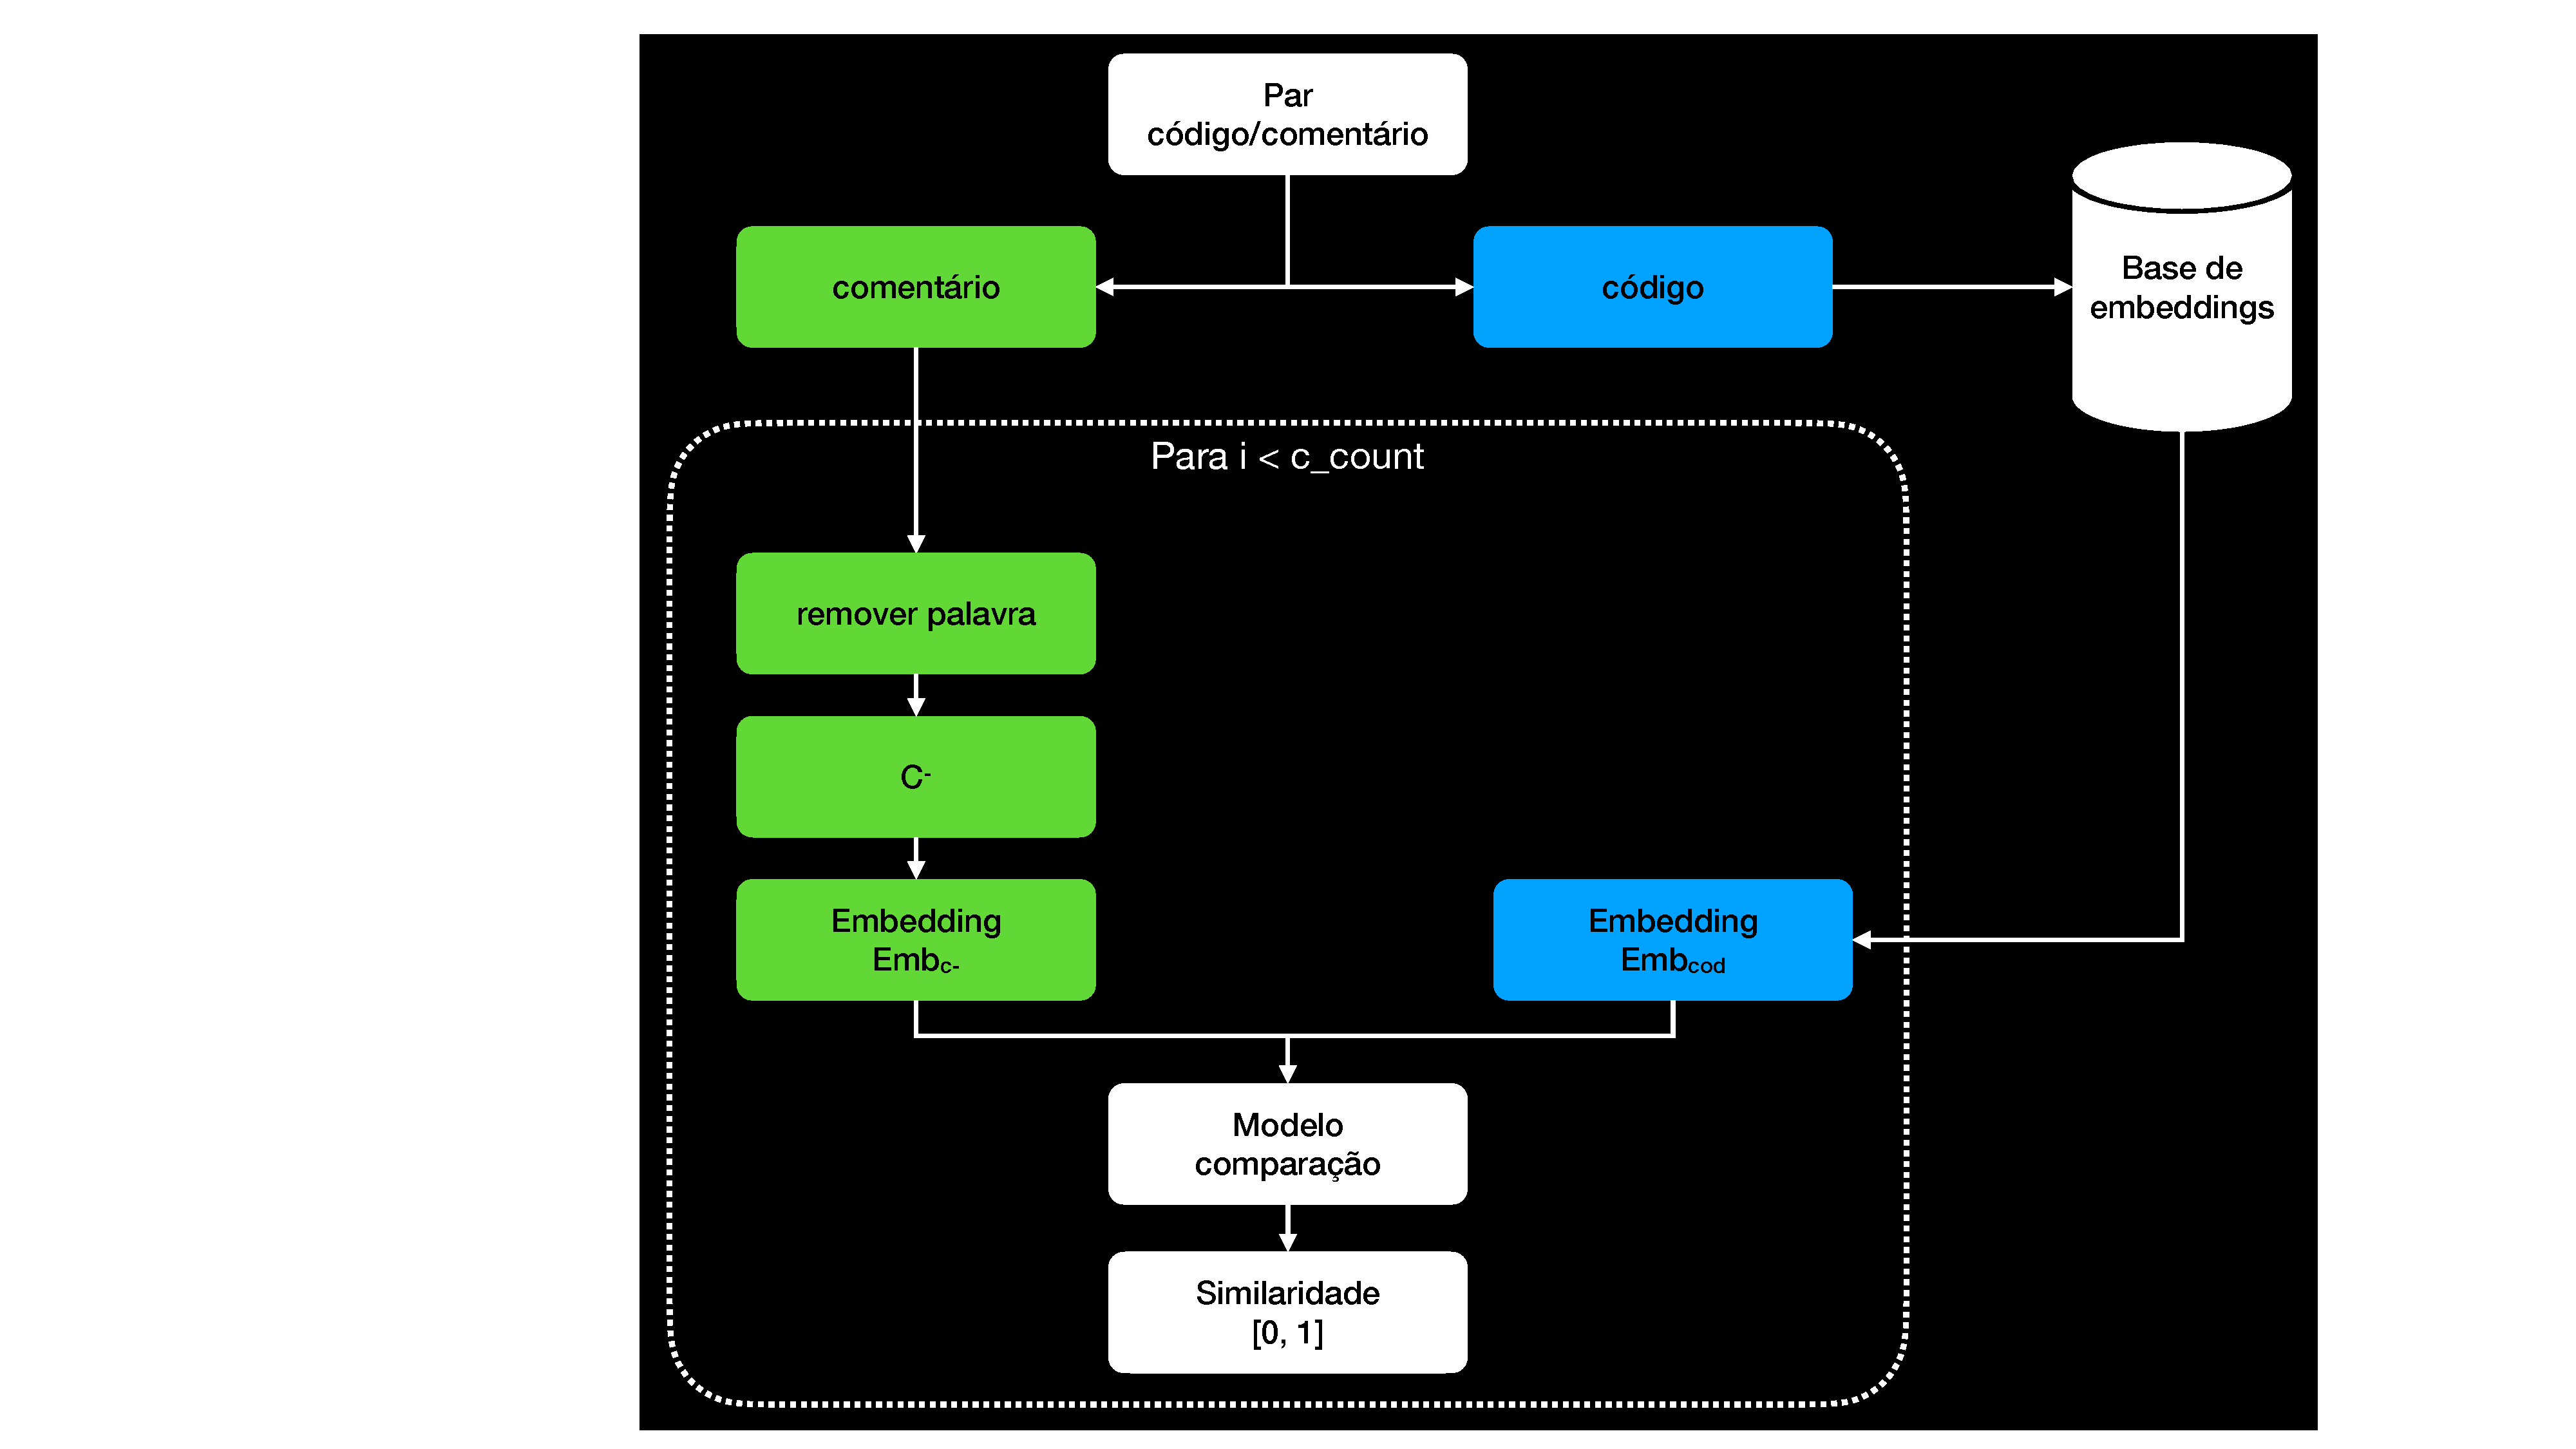
\includegraphics[scale=0.3]{imagens/proposta-experimental/experiment-1.pdf}
        \smallcaption{Fonte: Autor.}
        \label{fig:experiment-1-diagram}
\end{figure}

Para este experimento, espera-se que, ao remover uma palavra semanticamente importante para o par código/comentário, a similaridade seja baixa. De igual modo, quando uma palavra menos importante for removida, espera-se que a similaridade seja alta.

\section{Experimento 2}
\label{sec:experiments:experiment-2}
O objetivo desse experimento é determinar a relevância de determinada palavra no contexto de busca de código-fonte a partir de linguagem natural.

Neste experimento, foram utilizados os mesmos 100 pares da base de treinamento utilizados no experimento \ref{sec:experiments:experiment-1}, bem como o mesmo algoritmo de remoção de palavras de um comentário. Entretanto, ao invés de comparar o \textit{embedding} da \textit{query} $C^-$ com o \textit{embedding} de código do mesmo par, como no experimento \ref{sec:experiments:experiment-1}, este é aplicado ao contexto de busca de código-fonte a partir de linguagem natural.

A busca de código-fonte no presente trabalho é feita da seguinte forma: dado uma \textit{query} $Q$, é gerado um \textit{embedding} $Emb_q$ a partir da \textit{query} $Q$. Depois, para cada \textit{embedding} de código-fonte $Emb_{cod}$ presente na base de \textit{embeddings}, utiliza-se o modelo de comparação para determinar a similaridade entre $Emb_q$ e $Emb_{cod}$, gerando uma ranking de resultados, ordenado pela similaridade de forma decrescente. A Figura \ref{fig:metodology-system_overview} ilustra o processo de busca descrito, bem como a Figura \ref{fig:experiment-2-diagram} apresenta o diagrama do experimento em questão.

\begin{figure}[H]
    \centering
        \caption{Diagrama do experimento 2}
        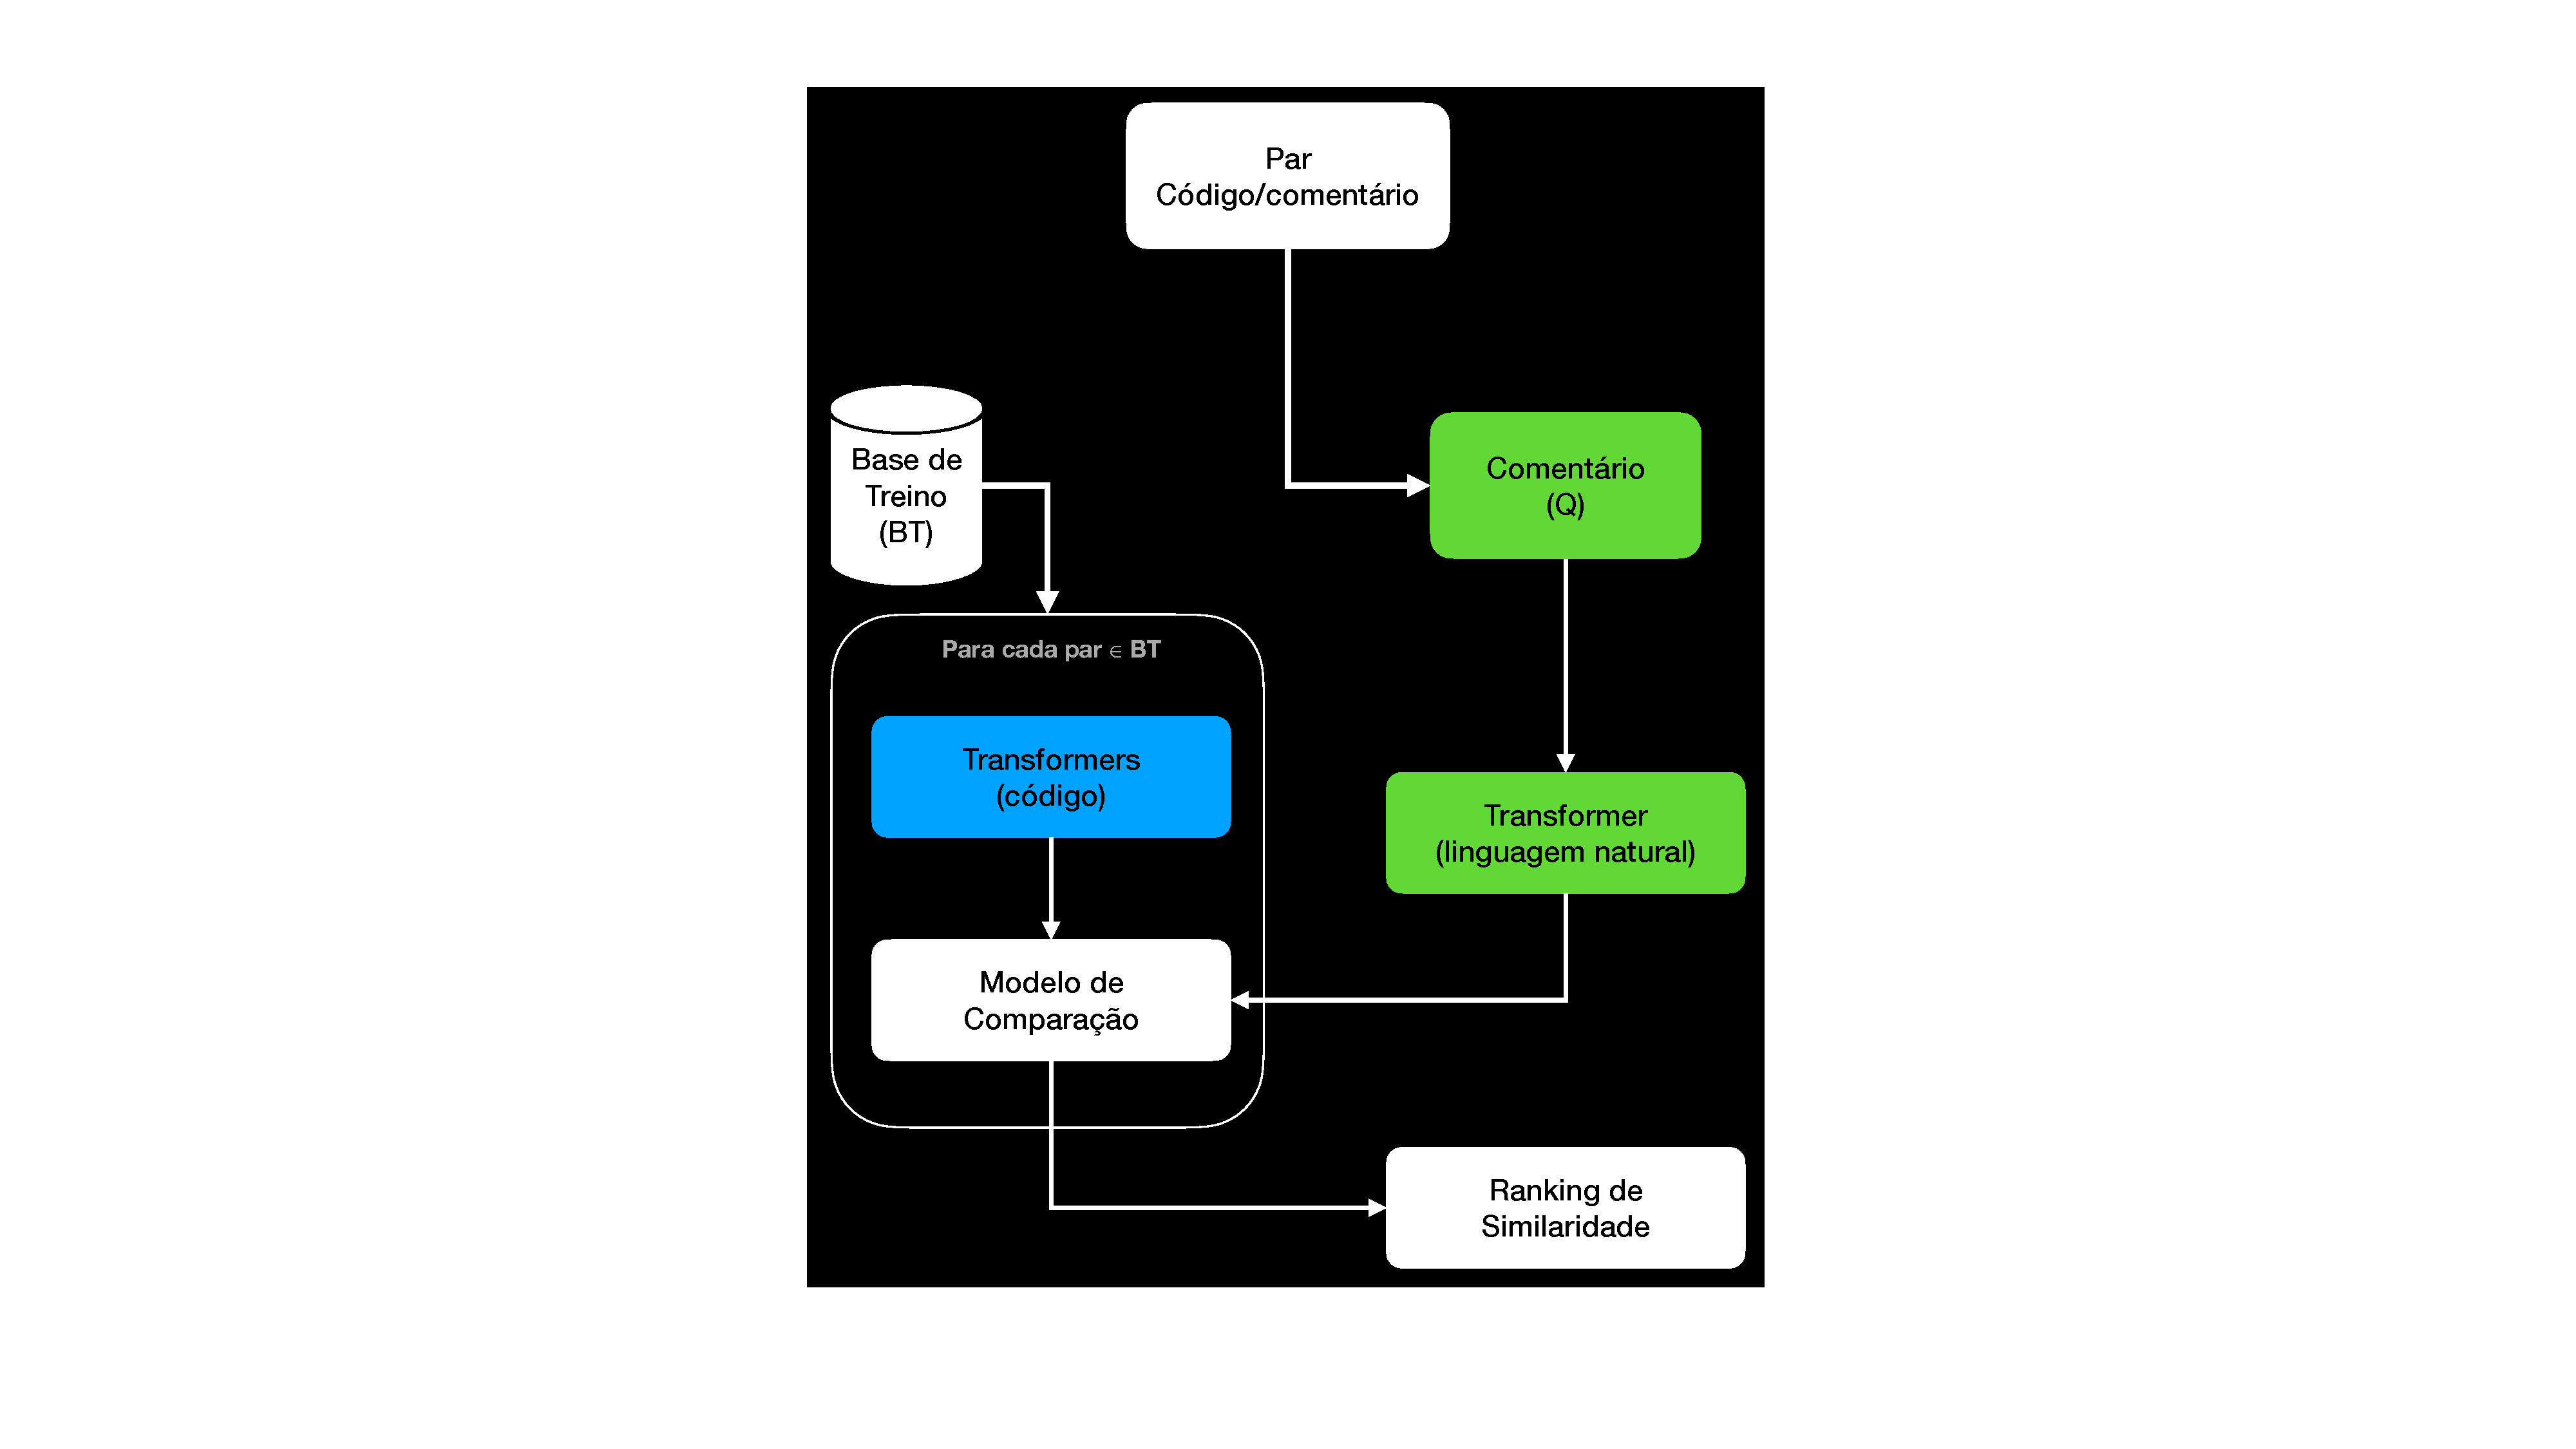
\includegraphics[scale=0.5]{imagens/proposta-experimental/experiment-2.pdf}
        \smallcaption{Fonte: Autor.}
        \label{fig:experiment-2-diagram}
\end{figure}

Nesse experimento, a \textit{query} $Q$ será o comentário do par em questão - não há portanto remoção de palavras como no experimento 1. Ainda, para avaliar a performance desse experimento, serão utilizadas as métricas \gls{mrr} e \textit{SuccessRate@k} com $k=1$, $k=5$ e $k=10$.

\section{Experimento 3}
\label{sec:experiments:experiment-3}
O objetivo desse experimento é determinar a acurácia do modelo de comparação, utilizando as queries disponíveis na base de dados \textit{CodeSearchNet}. Ao todo, a base em questão contém 4009 amostras, cada uma contendo os seguintes dados:

\begin{itemize}
    \item \textit{Query}: Termo, em linguagem natural, utilizado para busca de código-fonte. Para facilitar a compreensão, esse termo será chamado daqui em diante de $Q_{cs}$.
    \item \textit{Language}: Linguagem de programação do código-fonte associado
    \item \textit{GitHubUrl}: Link do Github para o código-fonte associado
    \item \textit{Relevance}: Valor inteiro, entre 0 e 3 (inclusivo), que representa o quão a \textit{Query} é relevante ao código-fonte em questão. 0 signfica que o código-fonte é pouco relevante para a query, e 3 signfica que o código é altamente relevante para a \textit{Query}.
    \item \textit{Notes}: Anotações, em linguagem natural, feitas pelos criadores dessa base de dados, caso julgassem relevante para a amostra em questão.
\end{itemize}

Para o experimento em questão, foram utilizadas apenas as amostras da linguagem \textit{Python}. Além disso, amostras duplicadas e aquelas cujo o campo \textit{GitHubUrl} não foi encontrado na base de treinamento também foram filtradas. Por fim, 842 amostras de \textit{queries} foram utilizadas neste experimento.

Portanto, para cada uma das amostras de query foi gerado um \textit{embedding} a partir de $Q_{cs}$, chamado $Emb_{qcs}$, utilizando o modelo de \textit{embedding} para linguagem natural \textit{all-mpnet-base-v2}, conforme descrito no capítulo \ref{chp:methodology}. Esse embedding foi então comparado com todos os embeddings $Emb_{cod}$ presentes na base de embeddings, utilizando o modelo de comparação.

Como o modelo de comparação proposto neste estudo gera resultados no intervalo $[0, 1]$, e o campo \textit{Relevance} possui valores inteiros entre 0 e 3, foi necessário uma normalização para determinar se o modelo categorizou o par $(Emb_{qcs}, Emb_{cod})$ de acordo com a relevância esperada. Para tanto, dividiu-se os dois intervalos ao meio. Com isso, para valores de \textit{Relevance} 0 ou 1, espera-se que a similaridade seja igual ou menor à 0.5, bem como para \textit{Relevance} 2 ou 3, espera-se similaridades maiores que 0.5. Como exemplo, caso a similaridade dada pelo modelo de comparacão for de $0.4$, e a relevância esperada para esta amostra seja 0, considera-se um acerto do modelo de comparação. Ainda, se a similaridade for $0.6$ e a relevância 1, considera-se um erro do modelo. Por fim, a Figura \ref{fig:experiment-3-diagram} ilustra o experimento em questão.

\begin{figure}[H]
    \centering
        \caption{Diagrama do experimento 3}
        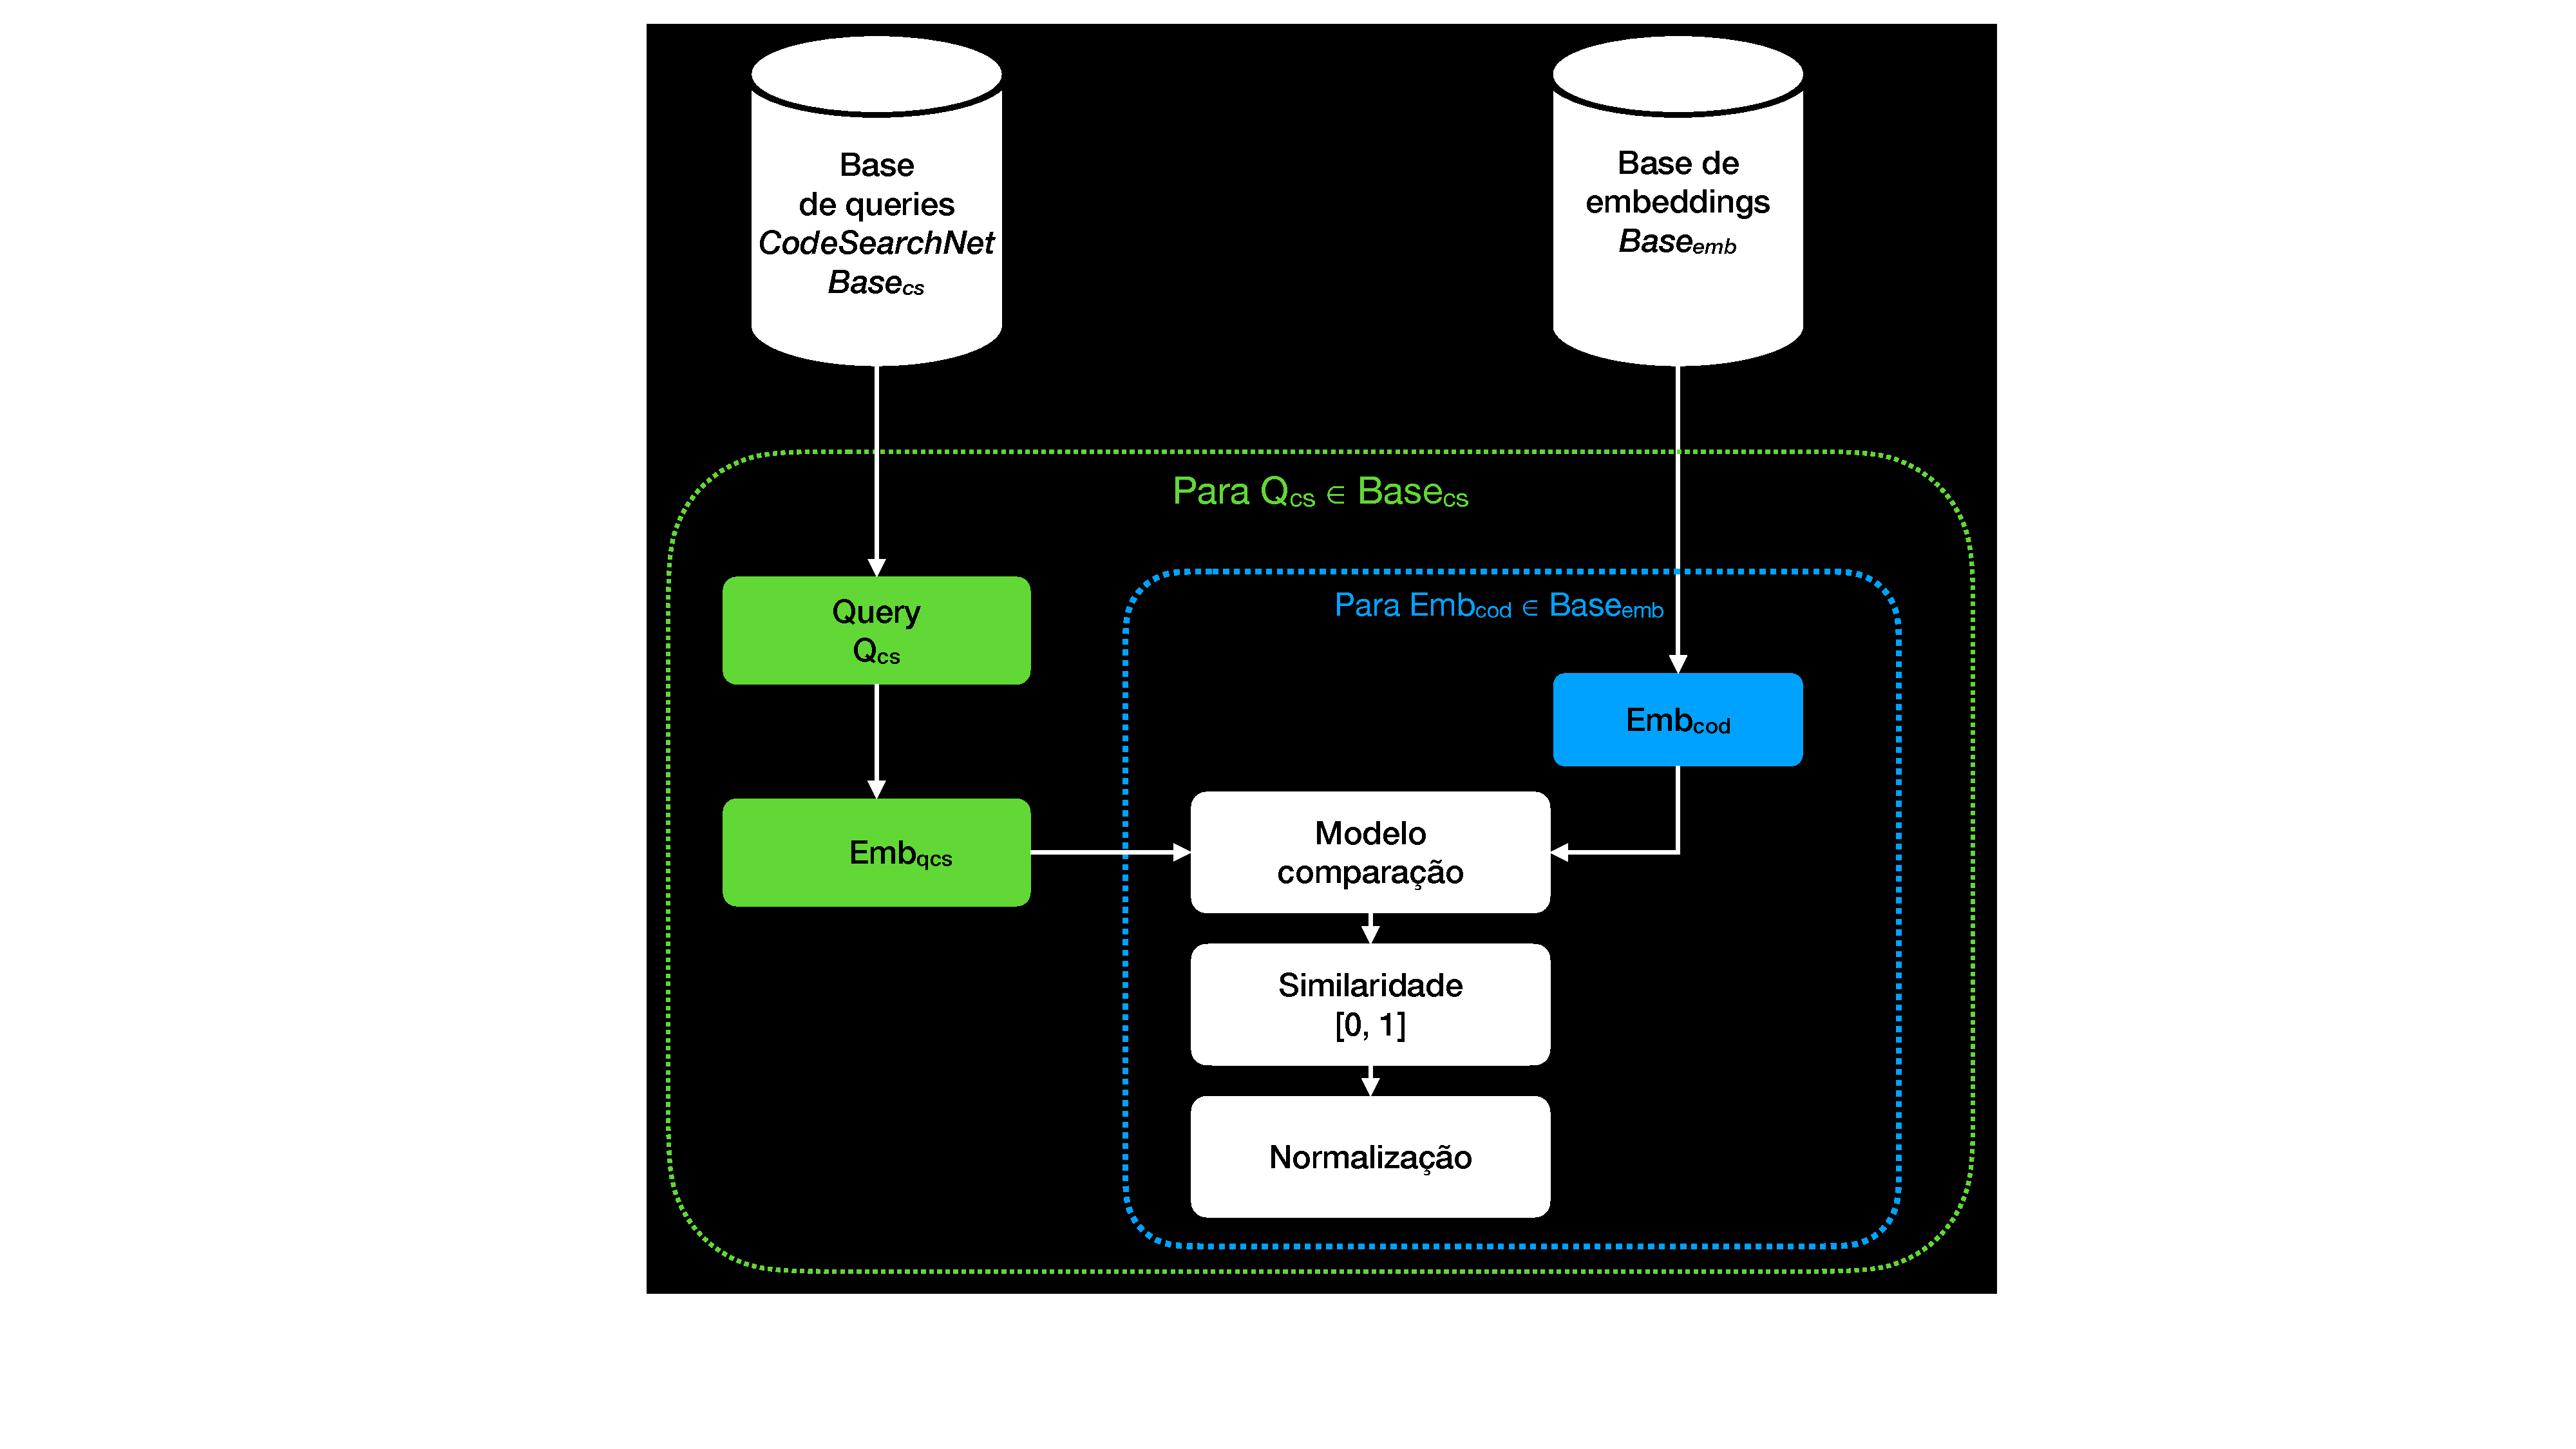
\includegraphics[scale=0.4]{imagens/proposta-experimental/experiment-3.pdf}
        \smallcaption{Fonte: Autor}
        \label{fig:experiment-3-diagram}
\end{figure}
